\subsection*{The Derivative of a Function}

\thispagestyle{empty}

The derivative of a function computes the slope of the tangent to a curve:

\begin{center}
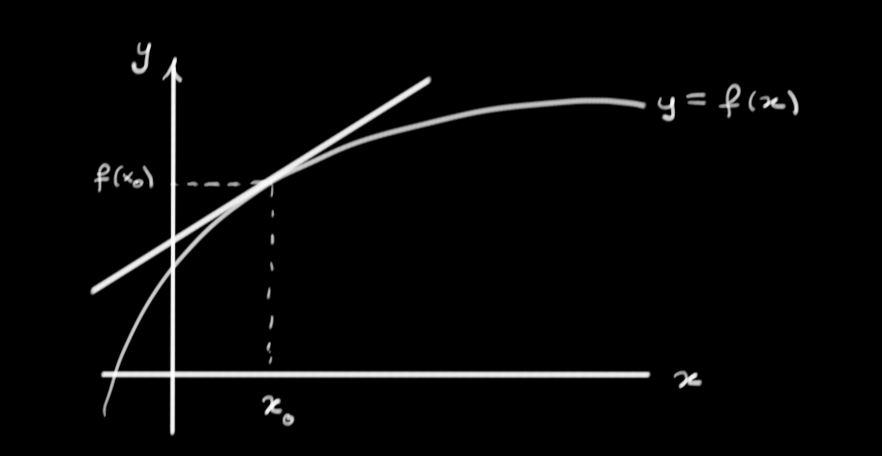
\includegraphics[scale=.4]{slope.jpg}
\end{center}

\noindent
To learn this concept watch this short movie:

\videoscriptlink{Derivative.mp4}{Derivative of a Function}{The Derivative}

\noindent
Now check that you watched carefully by taking this quiz:

\begin{center}
\href{\webworkurl Demo}{\raisebox{-3mm}{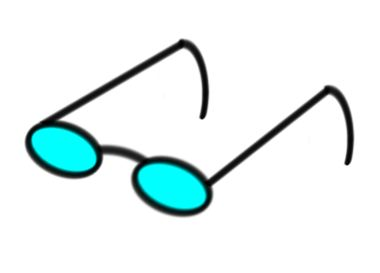
\includegraphics[scale=.1]{glasses.jpg}}\hspace{2mm} Derivative Quiz}\hspace{8mm}
\end{center}


\noindent{\bf Background Reading:}

\begin{itemize}
\item Thomas' Calculus: Chapter 2.7 {\em Tangents and Derivatives}
\item Calculus: Early Transcendentals: Chapter 2.1 {\em The Tangent and Velocity Problems}
\end{itemize}

\noindent{\bf Other Resources:}
\begin{itemize}
\item Wikipedia, \href{http://simple.wikipedia.org/wiki/Derivative_(mathematics)}{Derivative (mathematics)}
\item MIT OCW, \href{http://ocw.mit.edu/courses/mathematics/18-01-single-variable-calculus-fall-2006/video-lectures/lecture-3-derivatives/}{Lecture 3 Derivatives}
\end{itemize}


\newpage

%%%Insert this to get the typewriter font so it looks like a real movie script
{\ttfamily
\fontdimen2\font=0.4em
\fontdimen3\font=0.2em
\fontdimen4\font=0.1em
\fontdimen7\font=0.1em
\hyphenchar\font=`\-



\section*{Script: Derivative of a Function}

\thispagestyle{empty}

%%%%put a hypertarget around the opening bit of text

\hypertarget{The Derivative}{The} intuition for the derivative of a function at a point is  
a measure of the instantaneous rate of change of a function. In other words, it generalizes
the slope of a line to a non-linear function. 

Lets sketch an example. Consider $y=f(x)$ and think about the slope at a point $x_0$ where the function
equals $f(x_0)$. Then take another point $x_0+h$, a distance $h$ away, where the function is $f(x_0+h)$.
Now we can draw a line connecting the two points $(x_0,f(x_0))$ and $(x_0+h,f(x_0+h))$. This looks like this:

\begin{center}
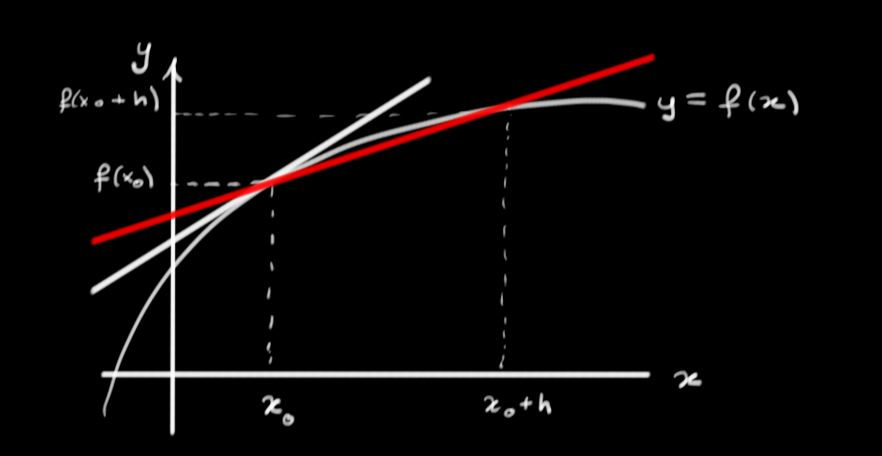
\includegraphics[scale=.4]{slope_red.jpg}
\end{center} 
 
\noindent 
The slope of the red line is
\[
\frac{f(x_0+h)-f(x_0)}{x_0+h-x_0}=\frac{f(x_0+h)-f(x_0)}{h}\, .
\] 

If we are trying to get a measurement of the slope of the curve at $x_0$, it makes sense to take points $x_0+h$
close to $x_0$. Intuitively speaking this means that we really want to use $h=0$ in this formula. There are two problems 
with this. First, if $h=0$, we are just looking at one point so we can't draw a line through two points anymore. The other problem
is that if you just look at the formula, setting $h=0$ means dividing by $h=0$ which makes no sense.


\newpage
\thispagestyle{empty}

But we have been studying limits in this course, so we know it does make sense to study the limit $h\to 0$. So we make a definition:
}
\begin{definition}
The derivative of the function $f(x)$, denoted by $f'(x)$, at the point $x$ is
\[
f'(x)=\lim_{h\to 0}\frac{f(x+h)-f(x)}{h}\, ,
\]
provided that the limit exists.
\end{definition}



\newpage